% Flattened output layout — didactic figure for the Aho-Corasick output emission.
% Standalone source. Compile with: pdflatex flattened-output.tex
% (uses Helvetica as an Arial stand-in so it matches the thesis sans look).
\documentclass[border=10pt]{standalone}
\usepackage[T1]{fontenc}
\usepackage{helvet}
\renewcommand{\familydefault}{\sfdefault}
\usepackage{tikz}
\usetikzlibrary{arrows.meta,positioning,calc,decorations.pathreplacing,fit}

\definecolor{idpblue}{HTML}{005DAA}
\definecolor{idpcyan}{HTML}{00B3FF}
\definecolor{warm}{HTML}{D7263D}
\definecolor{inkgray}{HTML}{444444}

\begin{document}
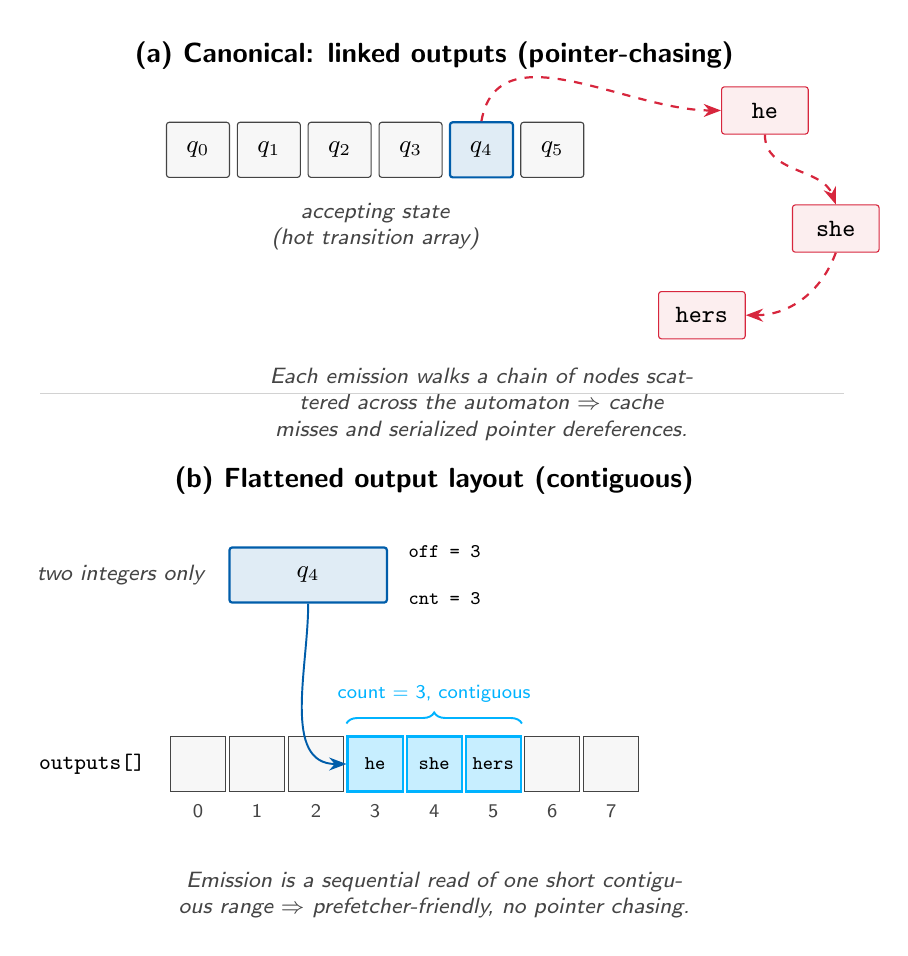
\begin{tikzpicture}[
    font=\small,
    >={Stealth[length=2.2mm]},
    state/.style={draw=inkgray, rounded corners=1pt, minimum width=8mm,
                  minimum height=7mm, inner sep=1pt, fill=gray!6},
    accept/.style={state, draw=idpblue, line width=0.8pt, fill=idpblue!12},
    cell/.style={draw=inkgray, minimum width=7mm, minimum height=7mm,
                 inner sep=1pt, fill=gray!6},
    seg/.style={cell, draw=idpcyan, line width=0.8pt, fill=idpcyan!22},
    pat/.style={draw=warm, rounded corners=1pt, minimum width=11mm,
                minimum height=6mm, inner sep=1pt, fill=warm!8},
    title/.style={font=\bfseries},
    note/.style={font=\footnotesize\itshape, text=inkgray, align=center},
    chain/.style={warm, line width=0.8pt, dashed},
]

% =====================================================================
% (a) CANONICAL: pointer-chasing
% =====================================================================
\node[title] at (3.0,2.6) {(a) Canonical: linked outputs (pointer-chasing)};

% hot state strip
\foreach \i [count=\n from 0] in {q_0,q_1,q_2,q_3,q_4,q_5} {
    \node[state] (sa\n) at (\n*0.9,1.4) {$\i$};
}
\node[accept] (sacc) at (4*0.9,1.4) {$q_4$};
\node[note, anchor=north] at (2.25,0.85) {accepting state\\(hot transition array)};

% scattered pattern nodes (deliberately misaligned -> "scattered")
\node[pat] (pa) at (7.2,1.9) {\texttt{he}};
\node[pat] (pb) at (8.1,0.4) {\texttt{she}};
\node[pat] (pc) at (6.4,-0.7) {\texttt{hers}};

% pointer chain from accepting state across memory
\draw[chain,->] (sacc.north) to[out=80,in=180] (pa.west);
\draw[chain,->] (pa.south) to[out=-90,in=110] (pb.north);
\draw[chain,->] (pb.south) to[out=-110,in=0]  (pc.east);

\node[note, anchor=north, text width=6.4cm] at (3.6,-1.25)
    {Each emission walks a chain of nodes scattered across the automaton
     $\Rightarrow$ cache misses and serialized pointer dereferences.};

% =====================================================================
% (b) FLATTENED: contiguous output array
% =====================================================================
\begin{scope}[yshift=-5.4cm]
\node[title] at (3.0,2.6) {(b) Flattened output layout (contiguous)};

% accepting state now stores (offset, count)
\node[accept, minimum width=20mm] (fstate) at (1.4,1.4)
    {\,$q_4$\,};
\node[anchor=west, font=\scriptsize] at (2.55,1.7) {\texttt{off = 3}};
\node[anchor=west, font=\scriptsize] at (2.55,1.1) {\texttt{cnt = 3}};
\node[note, anchor=east] at (0.2,1.4) {two integers only};

% contiguous outputs[] array
\foreach \idx [count=\n from 0] in {0,1,2,3,4,5,6,7} {
    \node[cell] (c\n) at (\n*0.75,-1.0) {};
    \node[font=\scriptsize, text=inkgray] at (\n*0.75,-1.6) {\idx};
}
% highlight the segment off..off+cnt = 3,4,5
\node[seg] (c3) at (3*0.75,-1.0) {\scriptsize\texttt{he}};
\node[seg] (c4) at (4*0.75,-1.0) {\scriptsize\texttt{she}};
\node[seg] (c5) at (5*0.75,-1.0) {\scriptsize\texttt{hers}};
\node[anchor=east, font=\footnotesize\ttfamily] at (-0.55,-1.0) {outputs[]};

% arrow from state offset to start of segment
\draw[idpblue,->,line width=0.7pt] (fstate.south) to[out=-90,in=180] (c3.west);

% brace over the contiguous range
\draw[decorate, decoration={brace, amplitude=4pt}, idpcyan, line width=0.7pt]
    ($(c3.north west)+(0,0.15)$) -- ($(c5.north east)+(0,0.15)$)
    node[midway, above=4pt, font=\scriptsize, text=idpcyan]{count = 3, contiguous};

\node[note, anchor=north, text width=6.6cm] at (3.0,-2.25)
    {Emission is a sequential read of one short contiguous range
     $\Rightarrow$ prefetcher-friendly, no pointer chasing.};
\end{scope}

% divider
\draw[gray!35, line width=0.4pt] (-2.0,-1.7) -- (8.2,-1.7);

\end{tikzpicture}
\end{document}
